%%%%%%%%%%%%%%%%%%%%%%%%%%%%%%%%%%%%%%%%%
% Beamer Presentation
% LaTeX Template
% Version 1.0 (10/11/12)
%
% This template has been downloaded from:
% http://www.LaTeXTemplates.com
%
% License:
% CC BY-NC-SA 3.0 (http://creativecommons.org/licenses/by-nc-sa/3.0/)
%
%%%%%%%%%%%%%%%%%%%%%%%%%%%%%%%%%%%%%%%%%

\documentclass{beamer}

\mode<presentation> {

\usetheme{Madrid}

\setbeamertemplate{navigation symbols}{} % Remove the navigation symbols from the bottom of all slides
}

\usepackage{graphicx} % Allows including images
\definecolor{links}{HTML}{2A1B81}
\hypersetup{colorlinks,linkcolor=,urlcolor=links}

\graphicspath{ {./images/} }

%----------------------------------------------------------------------------------------
% TITLE PAGE
%----------------------------------------------------------------------------------------

\title[Pandas \& testing]{Pandas \& testing} % The short title appears at the bottom of every slide, the full title is only on the title page
\author{Carlos A Molina}
\date{March 25, 2021}

\begin{document}

\begin{frame}
\titlepage % Print the title page as the first slide
\end{frame}

\begin{frame}
\frametitle{Table of contents}
\tableofcontents % Throughout your presentation, if you choose to use \section{} and \subsection{} commands, these will automatically be printed on this slide as an overview of your presentation
\end{frame}

%----------------------------------------------------------------------------------------
% PRESENTATION SLIDES
%----------------------------------------------------------------------------------------

%------------------------------------------------
\section{Introduction} % Sections can be created in order to organize your presentation into discrete blocks, all sections and subsections are automatically printed in the table of contents as an overview of the talk
%------------------------------------------------

\begin{frame}

\frametitle{Python. Why is it called Python?}

  \begin{figure}
    \centering
    \href{http://www.python.org/doc/faq/general/\#why-is-it-called-python}
      {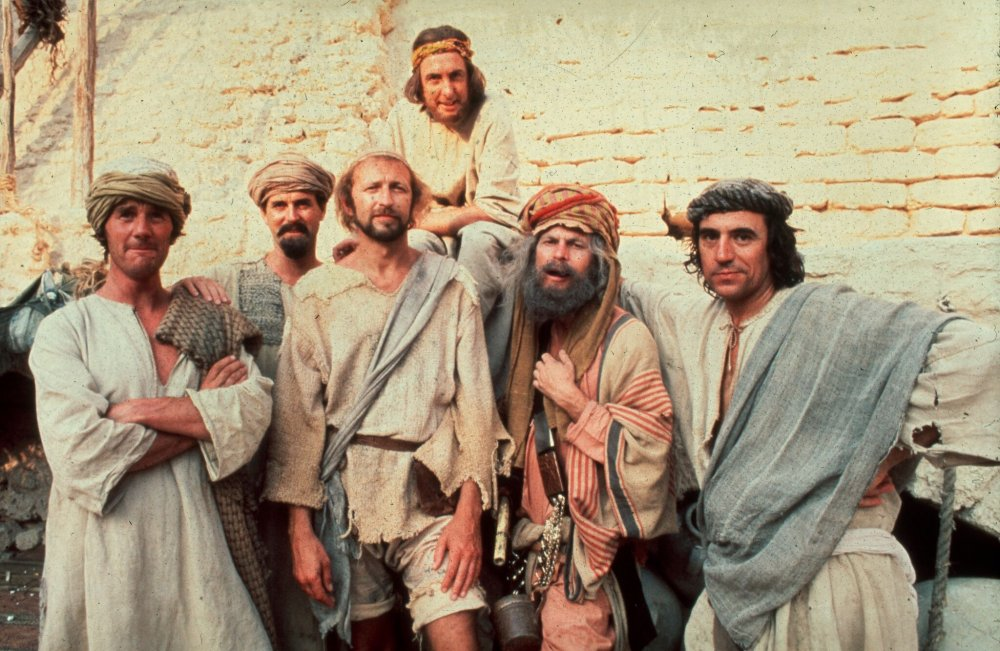
\includegraphics[width=0.9\textwidth]{brian.jpeg}}
  \end{figure}

\end{frame}

\begin{frame}

\frametitle{Extract Transform Load}

  \begin{figure}
    \centering
    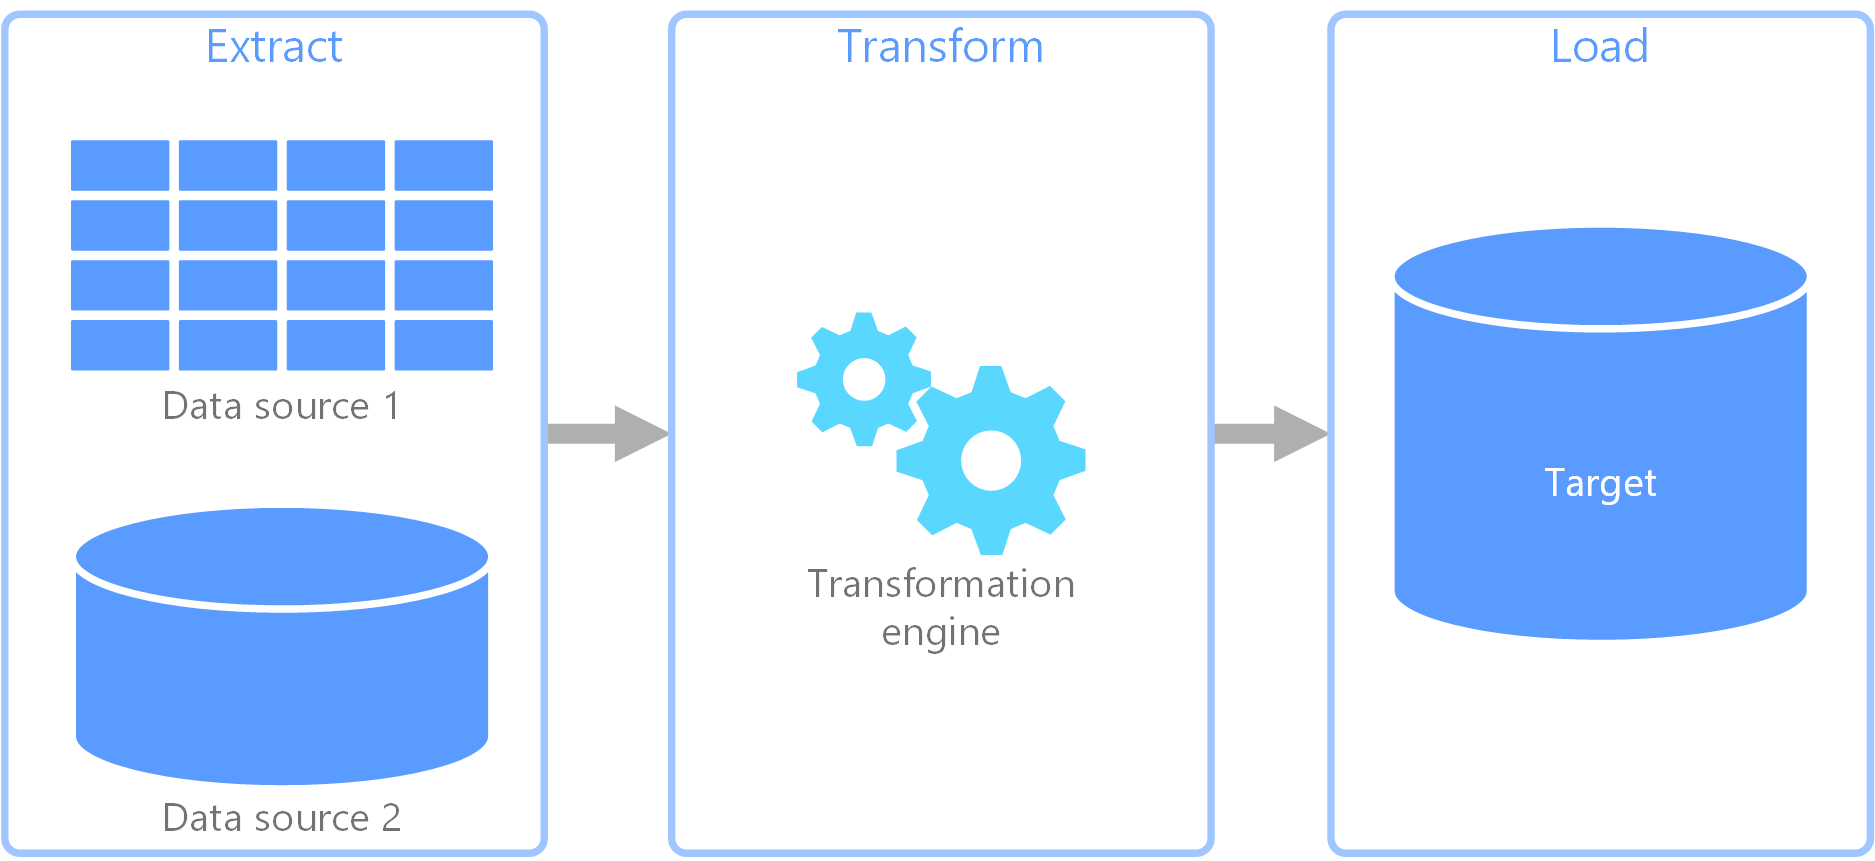
\includegraphics[width=\textwidth]{etl.png}
  \end{figure}

\end{frame}

\section{Demo}

\begin{frame}
\frametitle{Demo}

\begin{block}{Material}
\href{https://github.com/CarlosAMolina/workshop-python-pandas}{http://www.github.com/CarlosAMolina/workshop-python-pandas}
\end{block}

\begin{columns}[c] % The "c" option specifies centered vertical alignment while the "t" option is used for top vertical alignment

\column{.5\textwidth}
  \begin{figure}
    \centering
    
\includegraphics[width=0.7\textwidth]{olla.png}
  \end{figure}

\column{.45\textwidth}
\begin{itemize}
\item SQL VS Pandas
\item Pickle
\item Testing
\end{itemize}

\end{columns}

\end{frame}

\section{References}

\begin{frame}
\frametitle{References}
\begin{itemize}
\item BBVA Investment Funds\\
\href{https://www.bbva.es/personas/productos/fondos/por-tipo-de-activo.html}{https://www.bbva.es}
\item Docker MySQL\\
\href{https://hub.docker.com/\_/mysql/}{https://hub.docker.com}
\item LaTeX template\\
\href{https://www.latextemplates.com/template/beamer-presentation}{https://www.latextemplates.com}
\item MySQL export and import a database\\
\href{https://www.tutorialspoint.com/mysql/mysql-database-export.htm}{https://www.tutorialspoint.com}\\
\end{itemize}
\end{frame}

\begin{frame}
\frametitle{References}
\begin{itemize}
\item Presentation and material\\
\href{https://github.com/CarlosAMolina/workshop-python-pandas}{http://www.github.com/CarlosAMolina}
\item Python. Why is it called Python?\\
\href{http://www.python.org/doc/faq/general/\#why-is-it-called-python}{http://www.python.org}
\item SQLAlchemy\\
\href{https://docs.sqlalchemy.org/en/14/core/engines.html}{https://docs.sqlalchemy.org}
\end{itemize}
\end{frame}

\begin{frame}
\frametitle{References. Images}
\begin{itemize}
\item Cooking Pot\\
\href{https://pixabay.com/vectors/fire-flame-pot-burn-boil-stew-40252/}{https://pixabay.com}
\item ETL\\
\href{https://www.inetsoft.com/business/solutions/etl\_definition\_advantages\_and\_disadvantages/}{https://www.inetsoft.com}
\item Life of Brian\\
\href{https://www2.bfi.org.uk/news-opinion/news-bfi/announcements/bfi-announce-programme-its-monty-python-50}{https://www2.bfi.org.uk}
\end{itemize}
\end{frame}

\begin{frame}
\Huge{\centerline{Thank you!}}
\end{frame}

\end{document} 
